\documentclass{dense_template}
\newcommand*{\name}{Felipe Alejandro Jiménez Castillo}
\newcommand*{\code}{215671386}
\newcommand*{\school}{Universidad de Guadalajara - CUCEI}
\newcommand*{\course}{Computación Tolerante a Fallas}
\newcommand*{\assignment}{Hilos, procesos, demonios y concurrencia}
\renewcommand{\contentsname}{Contenido}

\begin{document}
\maketitle
%%%%%%%%%%%%%%%%%%%%
\tableofcontents
\newpage
%%%%%%%%%%%%%%%%%%%%
\section{Introducción}
Los hilos, procesos, demonios y concurrencia son conceptos fundamentales en la programación y la informática que se utilizan para administrar y ejecutar tareas de manera eficiente en sistemas computacionales.

\begin{itemize}
    \item \textbf{Procesos}
    \begin{itemize}
        \item Un proceso es un programa en ejecución independiente. Cada proceso tiene su propio espacio de memoria y recursos, lo que significa que no comparte memoria con otros procesos.
    \end{itemize}
    \begin{itemize}
        \item Los procesos pueden ser vistos como unidades independientes de trabajo que pueden realizar tareas por separado en un sistema operativo.
    \end{itemize}
    \begin{itemize}
        \item Los procesos pueden comunicarse entre sí utilizando mecanismos de comunicación interprocesos como tuberías o sockets.
    \end{itemize}
    \item \textbf{Hilos (threads)}
    \begin{itemize}
        \item Un hilo es una unidad más pequeña dentro de un proceso. Varios hilos pueden existir dentro de un solo proceso y comparten el mismo espacio de memoria y recursos del proceso padre.
    \end{itemize}
    \begin{itemize}
        \item Los hilos permiten una ejecución concurrente dentro de un proceso, lo que significa que múltiples tareas pueden ejecutarse en paralelo y compartir datos dentro del mismo proceso.
    \end{itemize}
    \begin{itemize}
        \item Los hilos son útiles para mejorar la eficiencia de la ejecución en sistemas multinúcleo o multitarea.
    \end{itemize}
    \item \textbf{Demonios (daemons)}
    \begin{itemize}
        \item Un demonio es un tipo especial de programa que se ejecuta en segundo plano en un sistema operativo sin interacción directa con un usuario.
    \end{itemize}
    \begin{itemize}
        \item Los demonios suelen realizar tareas de mantenimiento, administración o servicios en un sistema. Ejemplos comunes incluyen servidores web, servidores de correo y programas de copia de seguridad que se ejecutan en segundo plano.
    \end{itemize}
    \begin{itemize}
        \item Los demonios suelen iniciar su ejecución al arrancar el sistema y continuar ejecutándose durante toda la vida del sistema.
    \end{itemize}
    \item \textbf{Concurrencia}
    \begin{itemize}
        \item La concurrencia se refiere a la capacidad de un sistema para manejar múltiples tareas al mismo tiempo o en solapamiento.
    \end{itemize}
    \begin{itemize}
        \item Puede lograrse mediante el uso de procesos o hilos en un sistema. La concurrencia permite que múltiples tareas se ejecuten de manera aparentemente simultánea.
    \end{itemize}
    \begin{itemize}
        \item La programación concurrente puede mejorar el rendimiento y la capacidad de respuesta de una aplicación, pero también puede introducir problemas de sincronización y acceso a datos compartidos.
    \end{itemize}
\end{itemize}

\pagebreak
%%%%%%%%%%%%%%%%%%%%
\section{Desarrollo}
\subsection{¿Por qué se utiliza?}
La concurrencia se utiliza en los programas para hacer que el código se ejecute de forma más eficiente y efectiva. Esto se puede hacer ejecutando múltiples tareas al mismo tiempo, en lugar de secuencialmente. La concurrencia puede mejorar el rendimiento de los programas de varias maneras, incluyendo:

\begin{enumerate}
    \item Reducción del tiempo de espera: La concurrencia puede reducir el tiempo de espera de los usuarios al ejecutar varias tareas al mismo tiempo. Por ejemplo, un navegador web puede cargar una página web y descargar archivos al mismo tiempo, lo que reduce el tiempo que tarda el usuario en ver la página web completa.
    \item Mejora del rendimiento de las aplicaciones: La concurrencia puede mejorar el rendimiento de las aplicaciones que se realizan de forma intensiva en recursos. Por ejemplo, un servidor web puede procesar múltiples solicitudes de clientes al mismo tiempo, lo que mejora el rendimiento general del servidor.
    \item Posibilidad de nuevas aplicaciones: La concurrencia hace posible nuevas aplicaciones que no serían posibles sin ella. Por ejemplo, la transmisión de vídeo en vivo requiere que el vídeo se capture y se transmita al mismo tiempo, lo que no sería posible sin la concurrencia.
\end{enumerate}

La concurrencia también puede ser utilizada para mejorar la seguridad de los programas. Por ejemplo, un servidor web puede usar la concurrencia para distribuir las solicitudes de los clientes entre varios servidores, lo que hace que sea más difícil para un atacante violar el servidor.

\subsection{Aplicación}
Para la implementación de algún concepto de concurrencia dentro de la aplicación, primero valía la pena conceptualizar el problema a tratar con dicha temática. Para ello se tomo como base la resolución de diferentes llamadas a diferentes rutas de una aplicación web, donde una tarda más en ser servida y se queda a la espera de una respuesta de terceros, por lo que está retrasaría la resolución de la segunda petición.

\subsection{Solución}
Con esto en mente la solución se implemento, con respecto a la practica pasada, haciendo que exista un hilo especifico que sirva las respuestas de dicha ruta, de modo que el proceso principal (la aplicación como tal) no debe esperar a la resolución de dicha llamada.

 \begin{center}
    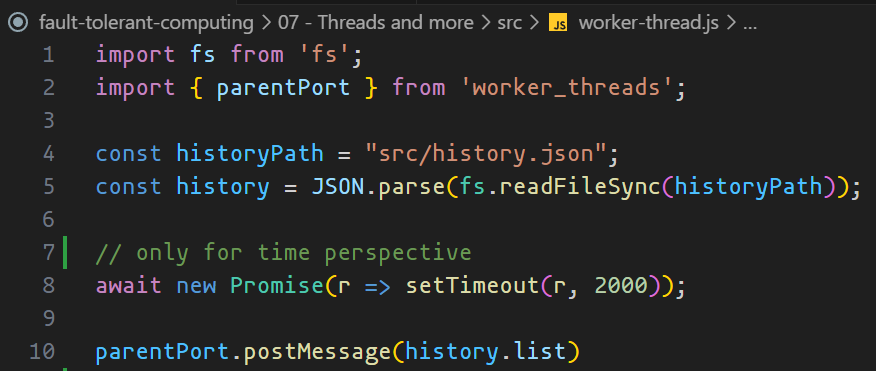
\includegraphics[width=0.9\textwidth]{thread-process.png}
    \vspace{1cm}
    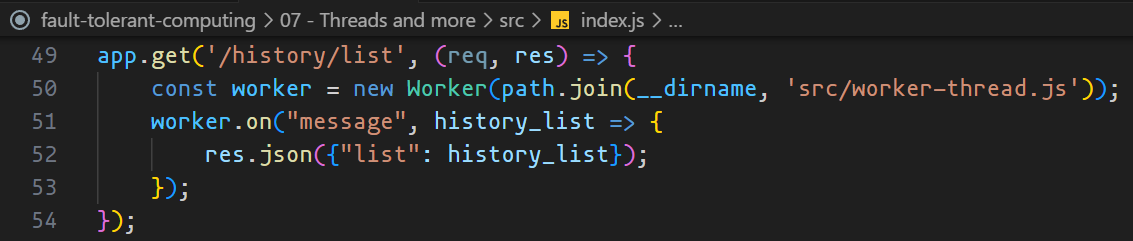
\includegraphics[width=0.9\textwidth]{route.png}
 \end{center}
%%%%%%%%%%%%%%%%%%%%
\pagebreak
%%%%%%%%%%%%%%%%%%%%
\section{Conclusión}
Es importante, siempre que se desarrolle una aplicación o servicio, tener en mente cómo y de qué forma funciona, ya que, como vimos en la proposición del problema, nuestra aplicación se puede ver afectada o reducida en capacidad de respuesta si no está bien implementada. Es por eso que los hilos, procesos, demonios y, en general, conceptos de concurrencia, son fundamentales para hacer que nuestras soluciones sean adecuadas y capaces, ya que no siempre se quedarán en la parte de desarrollo y en algún momento se verán enfrentadas a grandes cantidades de usuarios.  
%%%%%%%%%%%%%%%%%%%%
\pagebreak
%%%%%%%%%%%%%%%%%%%%
\section{Bilbiografia}
\sloppy
\begin{enumerate}
    \item Chillarege, R. (1996). Orthogonal defect classification. Handbook of software reliability engineering, 359-399.
    \item Myers, G. J., Sandler, C., \& Badgett, T. (2012). The art of software testing: Myers/art (G. J. Myers, T. Badgett, \& C. Sandler, Eds.). John Wiley \& Sons.
    \item Black, R. (2013). Managing the testing process: Practical tools and techniques for managing hardware and software testing. Wiley.
\end{enumerate}
\end{document}

